\documentclass{article}
\usepackage[T1]{fontenc}
\usepackage{lmodern}
\usepackage{graphicx}
\usepackage{amsmath,amssymb}
\usepackage[a4paper,margin=2cm]{geometry}
\usepackage[absolute,overlay]{textpos}
\setlength{\TPHorizModule}{1mm}
\setlength{\TPVertModule}{1mm}
\usepackage[indonesian]{babel}
\usepackage{hyperref}
\setlength{\emergencystretch}{2em}
% unit: Halaman 9

\begin{document}

% === Halaman 9 (llm) ===

\begin{center}
\Huge Steganografi
\end{center}

\vspace{60mm}

\begin{center}
\textcolor{red}{\large Stego-data tidak menimbulkan kecurigaan bagi pengamat \\
 Pesan yang tersembunyi di dalamnya tidak dapat dideteksi.}
\end{center}

% deskripsi: Ilustrasi konsep steganografi yang menunjukkan proses pengiriman pesan tersembunyi antara dua orang, dengan seorang pengamat yang menggunakan kaca pembesar namun tidak dapat mendeteksi pesan tersebut.
% bbox normalisasi: [0.1800, 0.2200, 0.8200, 0.7400]
\begin{textblock*}{134.40mm}(37.80mm,65.34mm)
\noindent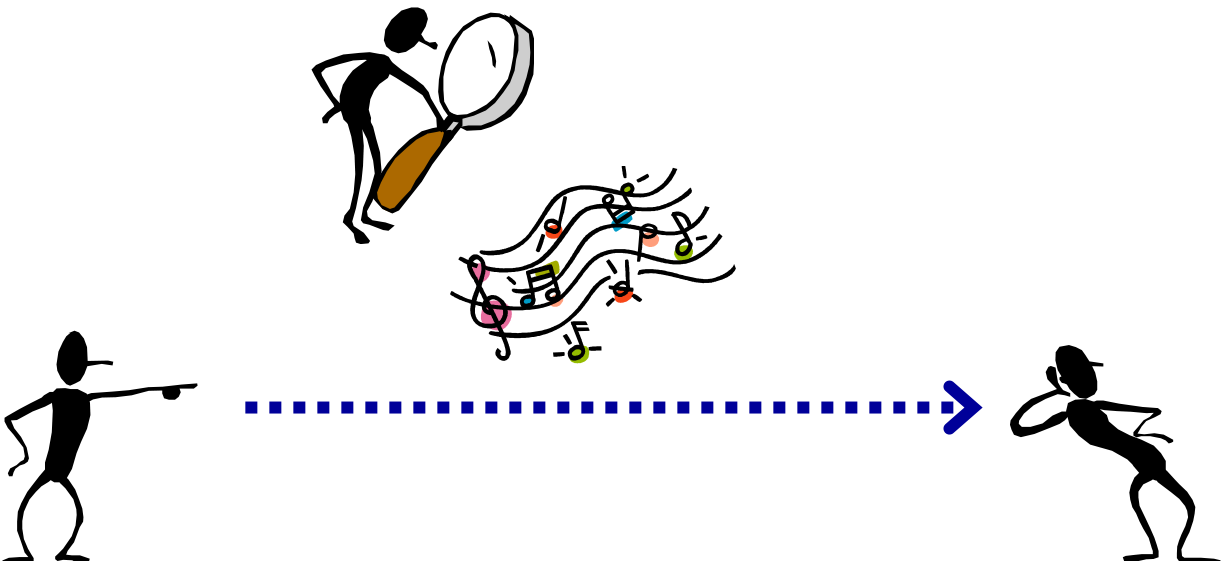
\includegraphics[width=134.40mm,height=154.44mm]{../../images/llm/page_009_img_01.png}%
\end{textblock*}

\end{document}
